\textbf{Problem definition}:
Write a program for fixed point continuation to generate both the stable and unstable branch of
%
\begin{equation}\label{eq:Q1_GE}
	\dot{x} = \mu - x^2
\end{equation}
%
\noindent\hrulefill

% -------------------------------------------------------------------
\textbf{Solution approach:}
We use sequential continuation for this problem. Each of the stable and unstable branches are tracked by starting from a location on them. It should be noted that due to the turning point at $\mu = 0$ we cannot get both branches using same initial point since we cannot got pass the turning point.

To track the stable branch, we choose our initial guess at $\mu_0 = 0.01$ and $x_0 = 0.1$. The $x$ value is then updated for new value of $\mu_1$ using the following equation.
%
\begin{equation}
	x_1^{k+1} = x_1^{k} + r \Delta x^k
\end{equation}
%
where we set $x_1^0$ equal to $x_0$. $r$ is the relaxation parameter that defines how much we can go in $\Delta x^k$ direction. For this problem, we chose $r$ and $0.1$. $\Delta x^k$ is calculated using the following formula.
%
\begin{equation}
	F_x \left( x_{j+1}^k, \mu_{j+1} \right) \Delta^k = 
	-F \left( x_{j+1}^k, \mu_{j+1} \right)
\end{equation}
%

where $k$ is the iteration number and $j+1$ is the index of the control parameter we are at. We iterate on $x$ until a convergence is satisfied. At the next fixed point, $x_{j+1}$ we know that the right-hand-side of Equation \eqref{eq:Q1_GE} is equal to zero. Therefore, we define the convergence criteria as $F(x, \mu) < 10^{-5}$. The solution of this approach is verified using the analytical results for the stable and unstable branches. These are calculated as follows.
%
\begin{equation}
\begin{cases}
	x = \sqrt{\mu} \quad \text{stable branch} \\
	x = -\sqrt{\mu} \quad \text{unstable branch}
\end{cases}
\end{equation}
%
The initial location for the stable branch is defined as $(x, \mu) = (0.01, 0.0001)$. The stable branch is followed for the $1000$ points between $\mu = 0.0001$ and $\mu = 10$. The convergence plots for $\mu = 1$ is shown in Figure \ref{fig:Q1_convergenceFORstable}. As shown here, the value of $F$ drops to zero when $x$ converges to its value of $1$ at $\mu = 1$.
%
\begin{figure}[h]
	\centering
	\begin{subfigure}[h]{8.0 cm}
		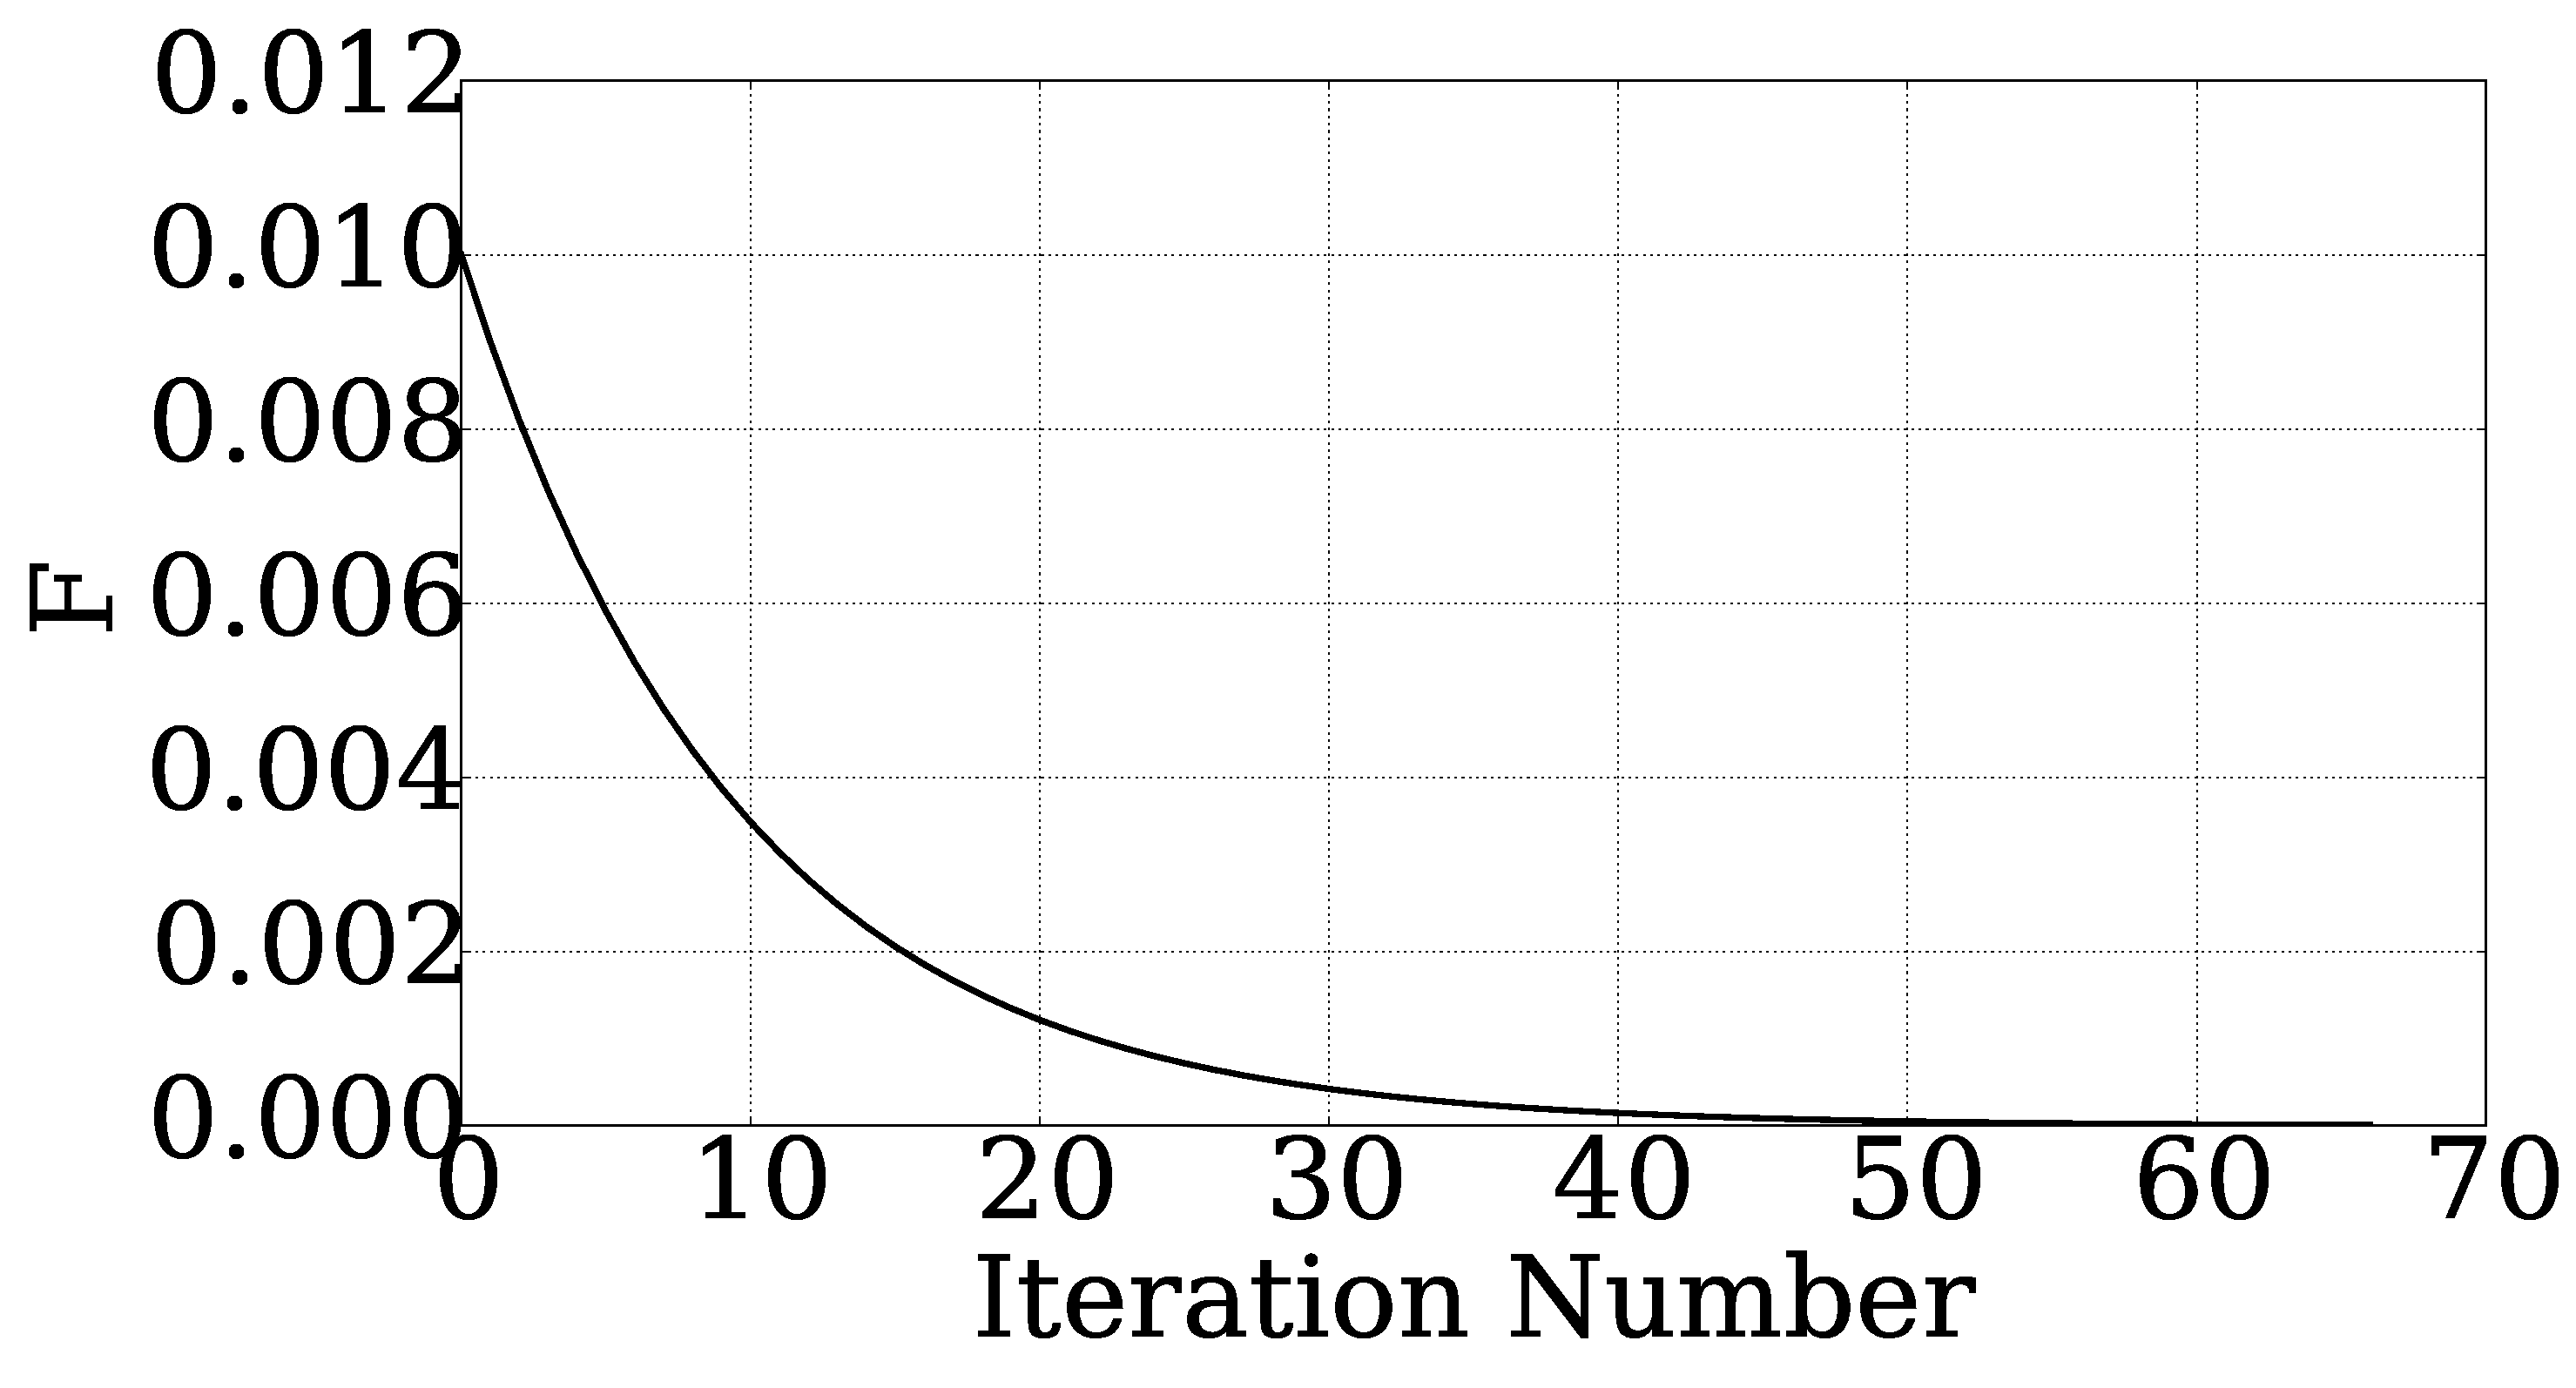
\includegraphics[width=8.0 cm]{figure/Q1/F_1.eps}
		\caption{Convergence of state equation, $F$}
	\end{subfigure}
	\begin{subfigure}[h]{8.0 cm}
        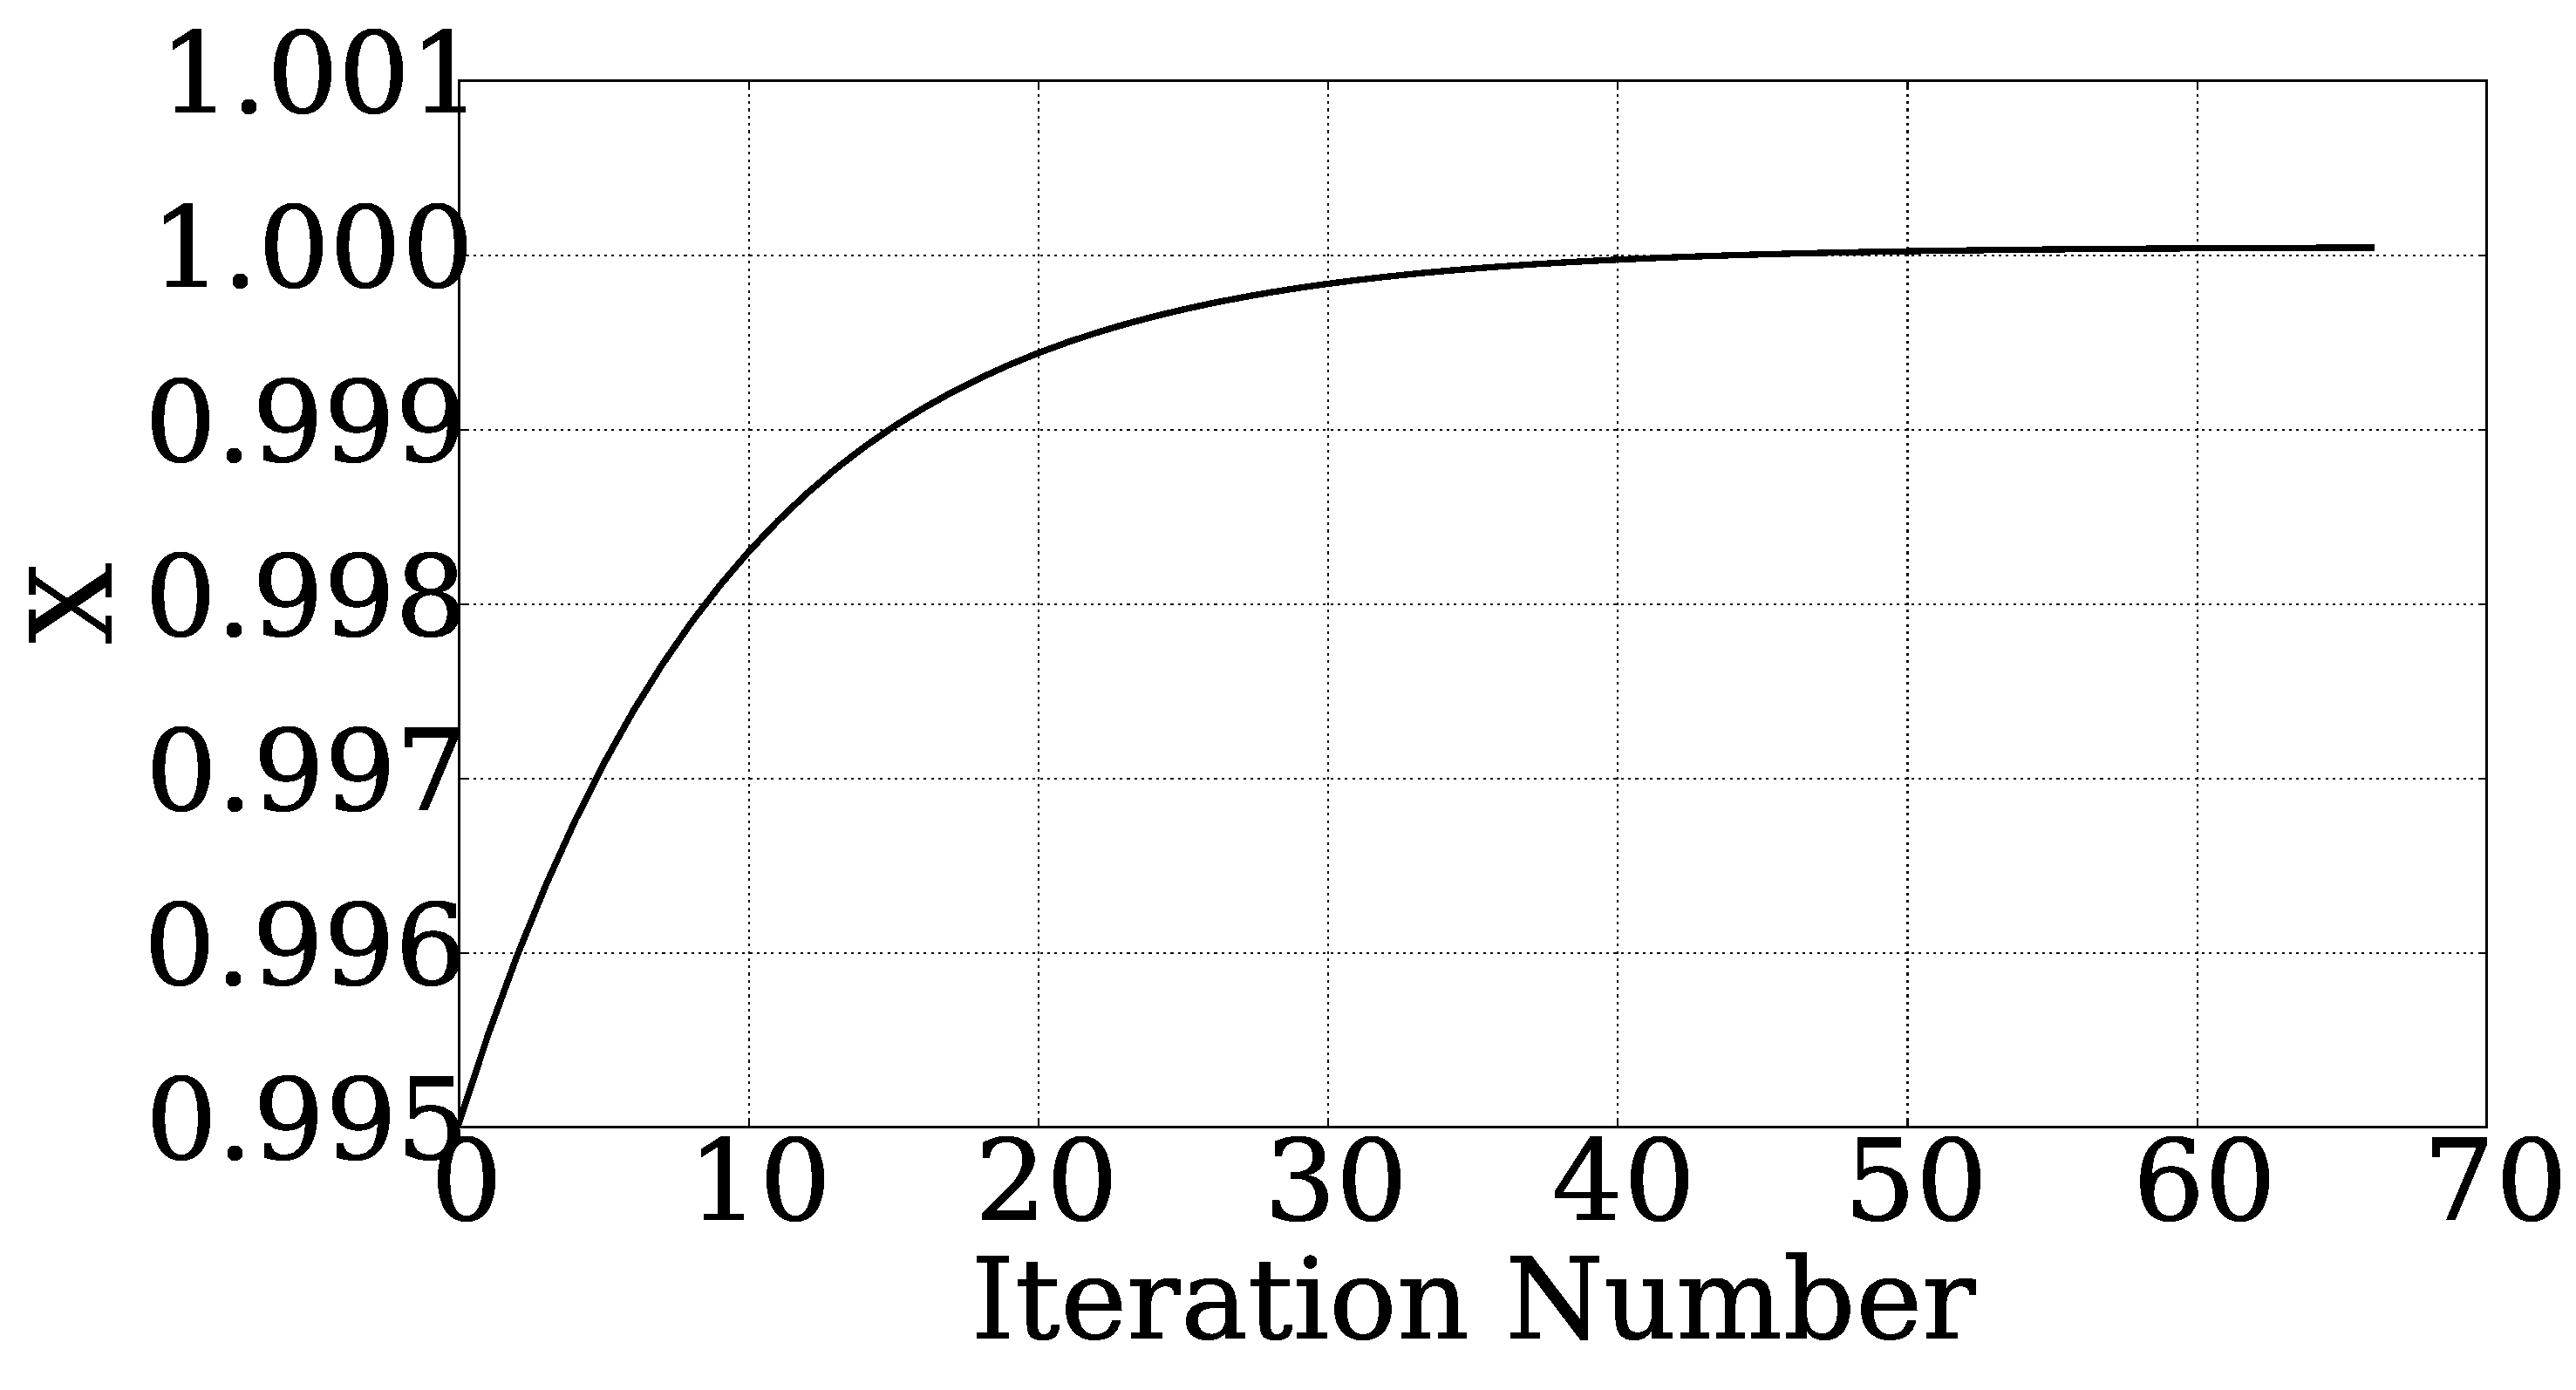
\includegraphics[width=8.0 cm]{figure/Q1/X_1.eps}
		\caption{Convergence of $x$ to its value.}
    \end{subfigure}
    \caption{Convergence plots for $x$ and $F$ for $\mu = 1$.}
    \label{fig:Q1_convergenceFORstable}
\end{figure}
%

The initial location for the unstable branch is defined as $(x, \mu) = (-0.01, 0.0001)$. The unstable branch is followed for the $1000$ points between $\mu = 0.0001$ and $\mu = 10$. The convergence plots for $\mu = 2$ is shown in Figure \ref{fig:Q1_convergenceFORunstable}. As shown here, the value of $F$ drops to zero when $x$ converges to its value of $-\sqrt{2}$ at $\mu = 2$.
%
\begin{figure}[h]
	\centering
	\begin{subfigure}[h]{8.0 cm}
		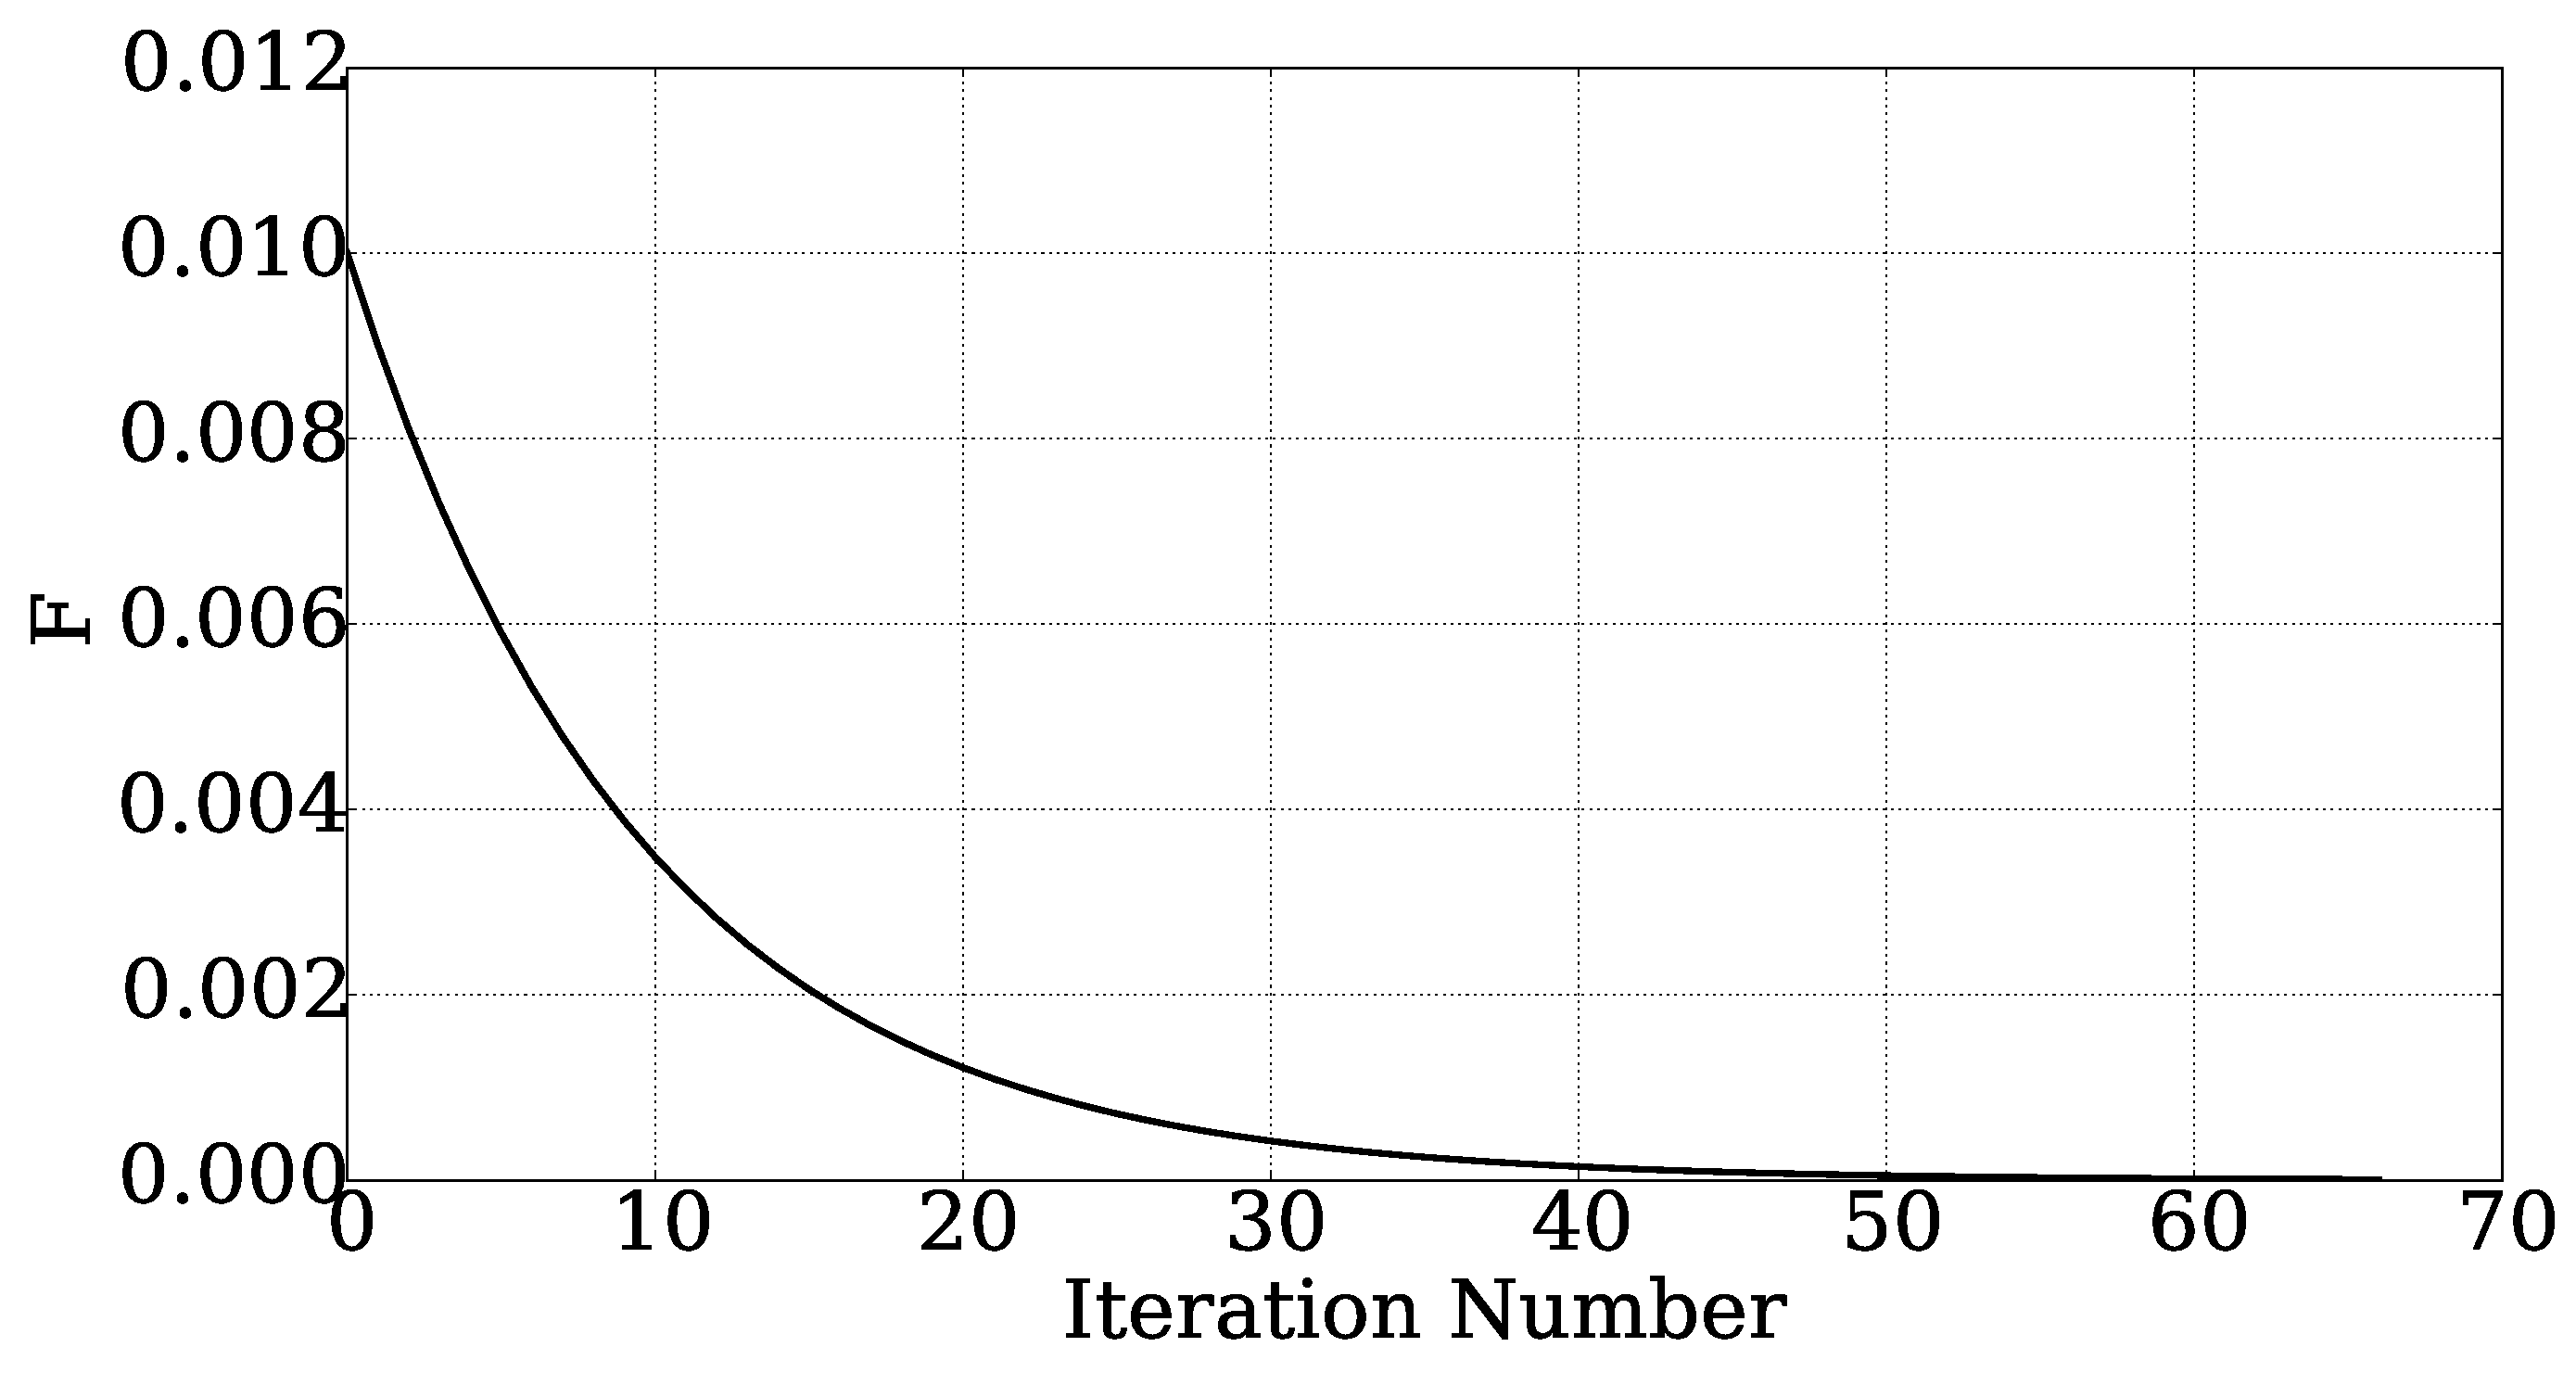
\includegraphics[width=8.0 cm]{figure/Q1/F_-2.eps}
		\caption{Convergence of state equation, $F$}
	\end{subfigure}
	\begin{subfigure}[h]{8.0 cm}
        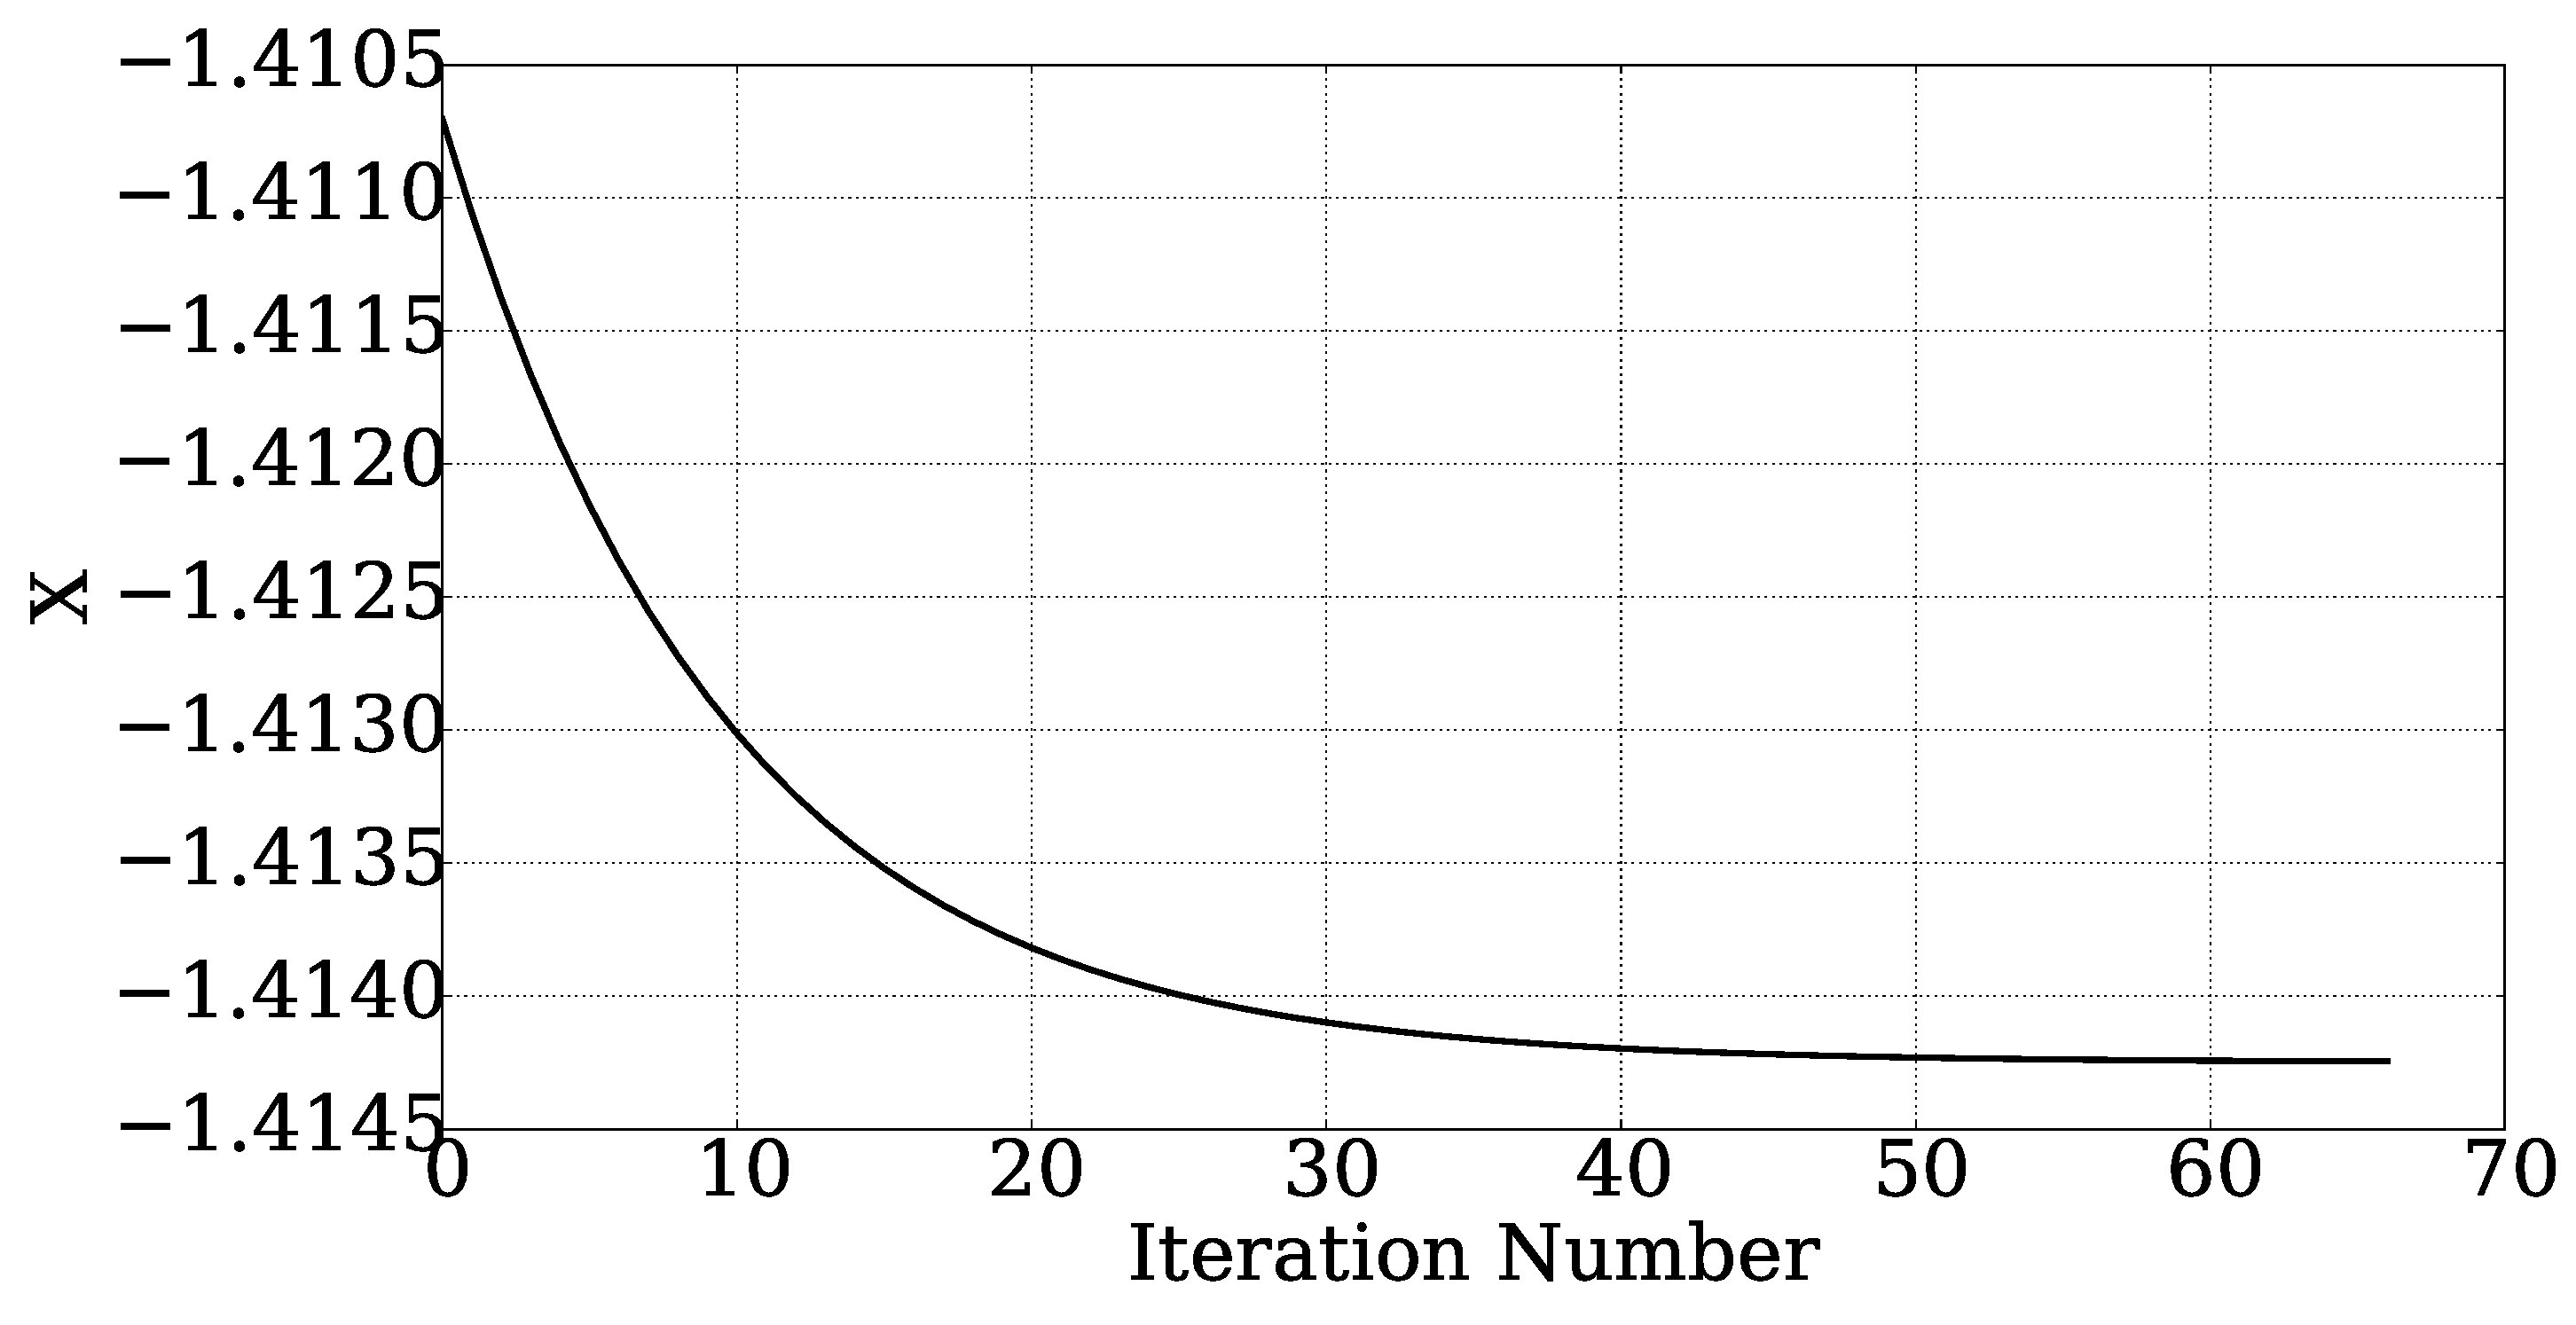
\includegraphics[width=8.0 cm]{figure/Q1/X_-2.eps}
		\caption{Convergence of $x$ to its value.}
    \end{subfigure}
    \caption{Convergence plots for $x$ and $F$ for $\mu = 2$.}
    \label{fig:Q1_convergenceFORunstable}
\end{figure}
%

The stable and unstable branch are shown in Figure \eqref{fig:Q1_branch}. The analytical results are represented using circles and the \emph{fixed point continuation} solution are shown with solid and dashed lines. The solid line represents the stable branch whereas the dashed line is used to show the unstable one.
%
\begin{figure}[h]
	\centering
	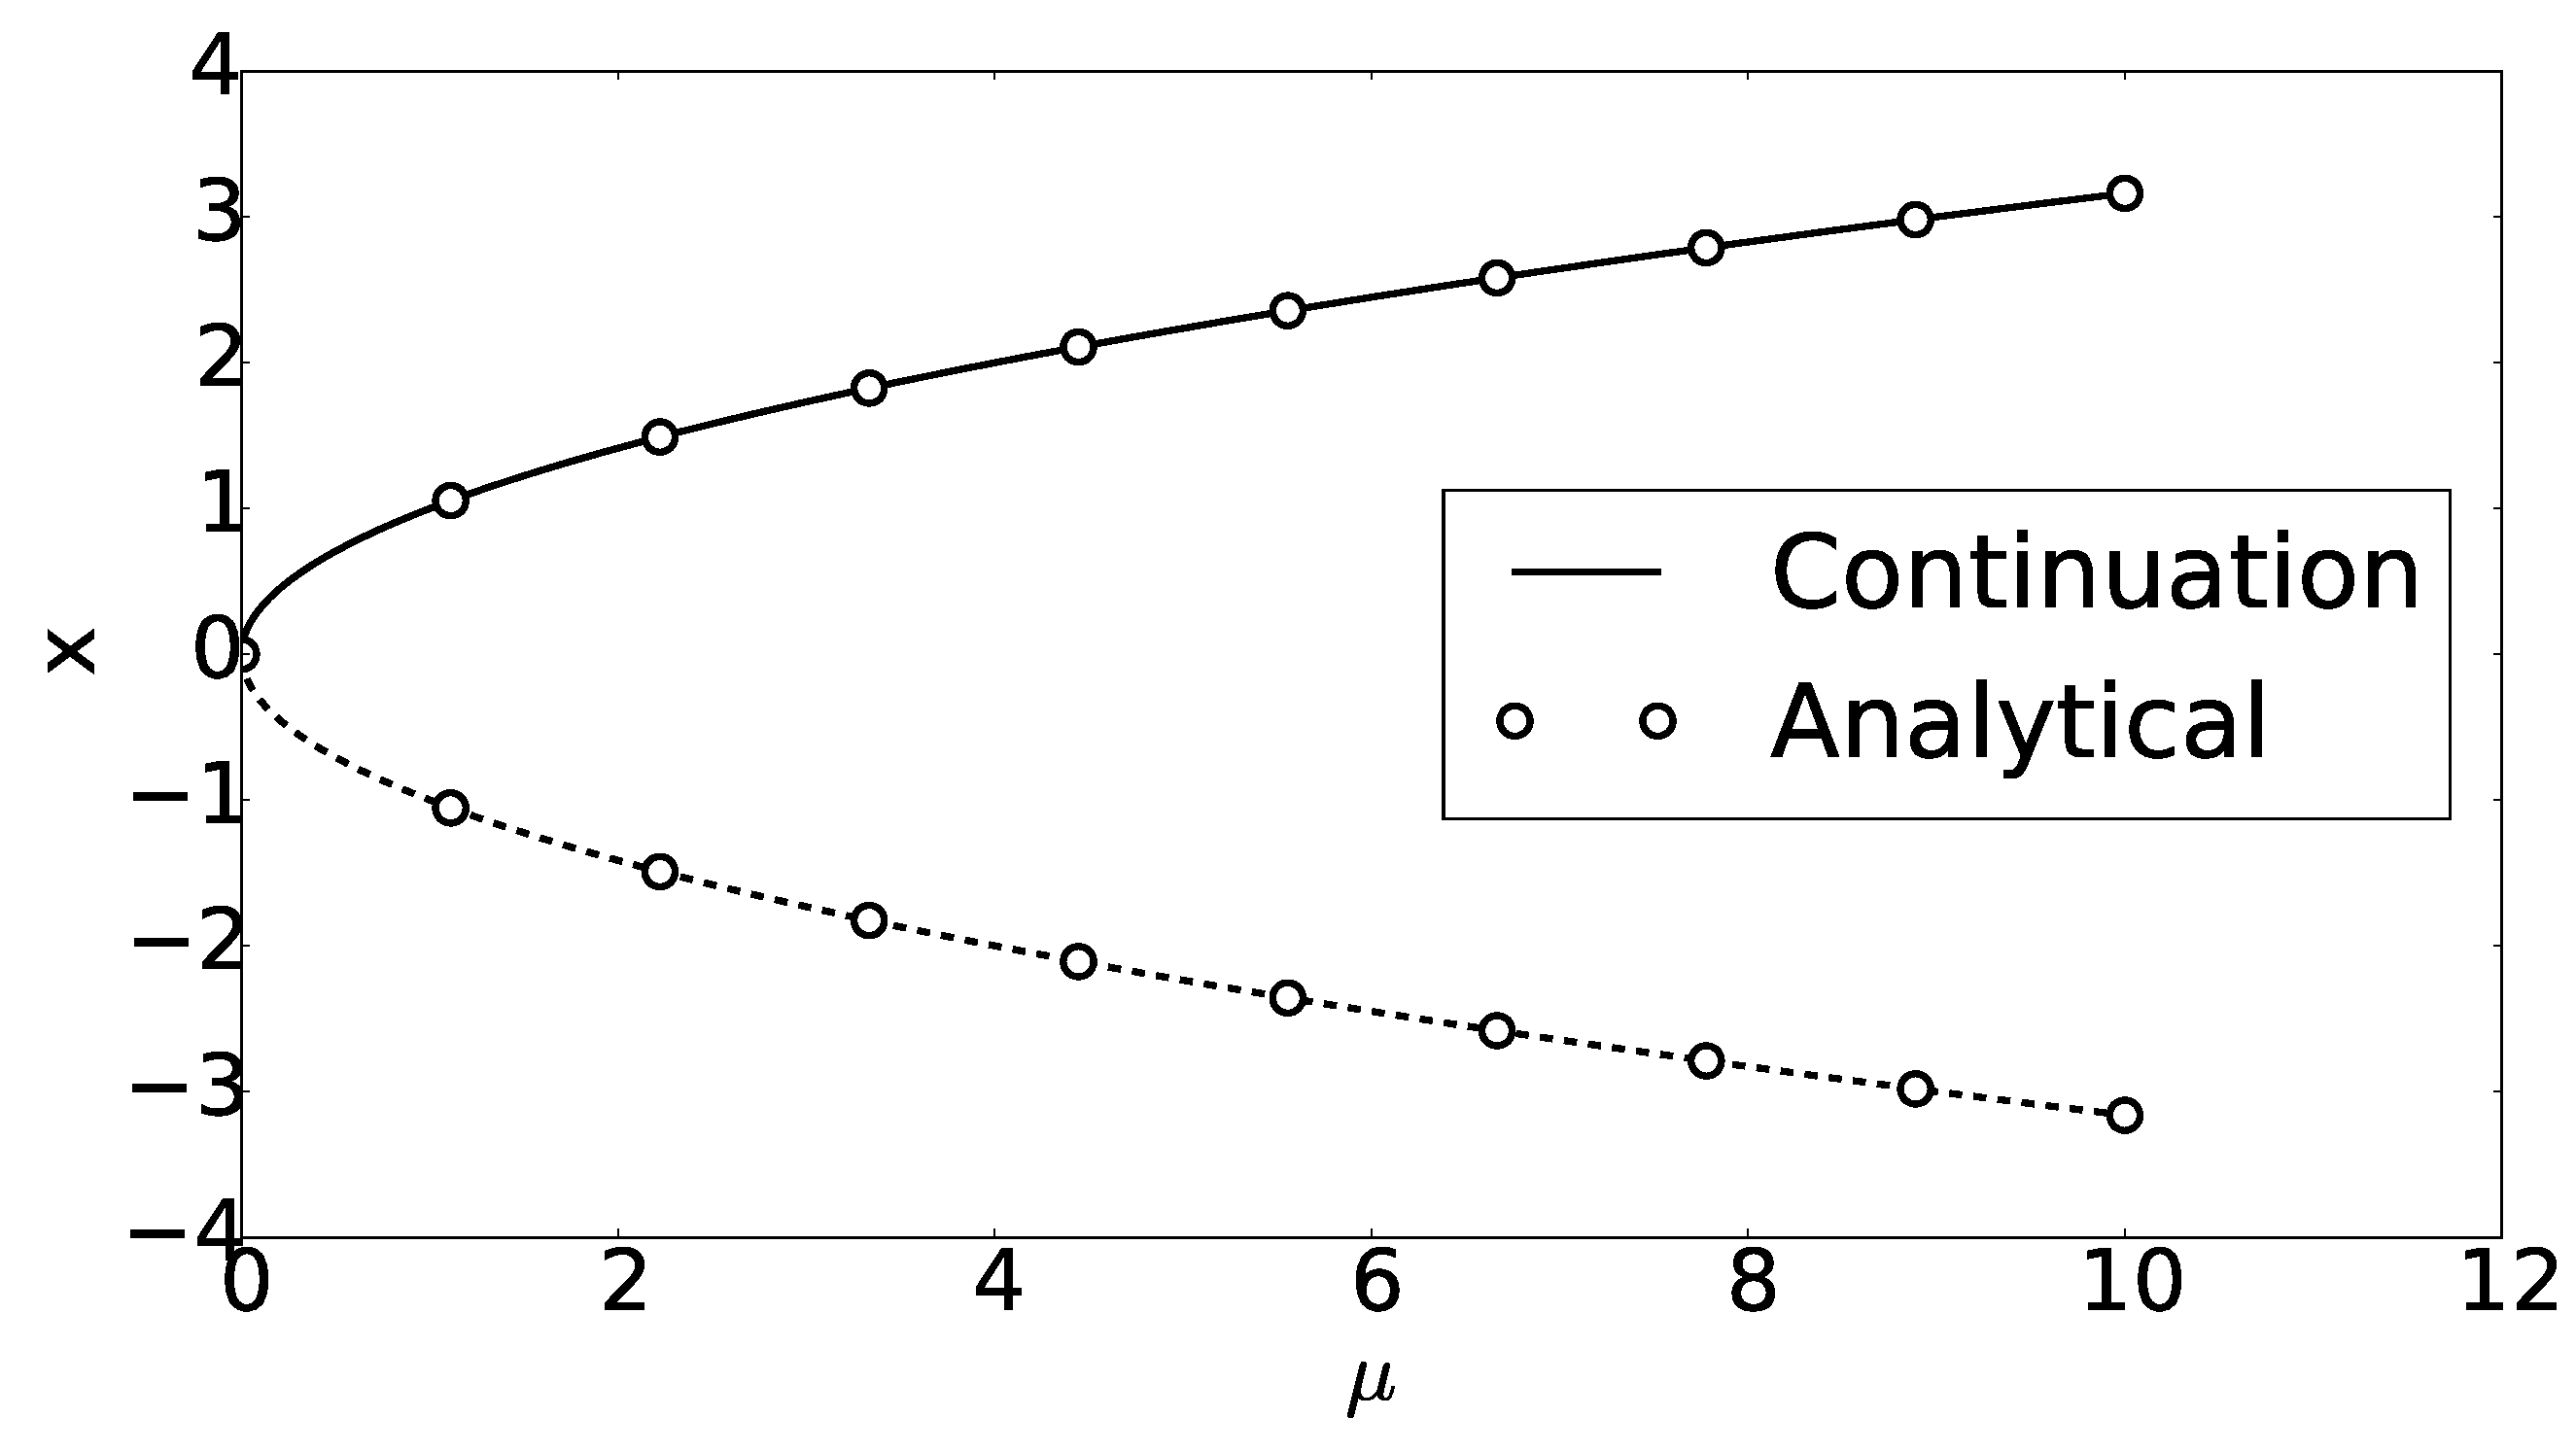
\includegraphics[width=12.0cm]{figure/Q1/bifurcation.eps}
	\caption{Comparison between fixed point continuation and analytical result for stable and unstable branches.}
	\label{fig:Q1_branch}
\end{figure}
%
The \texttt{Python} code for this problem is included at the end of the documentation for this problem.